\documentclass[../dissertation.tex]{subfiles}

\begin{document}
%%%%% COMPONENTS %%%%%
\section{Components}

Splitting up the project into multiple components has been useful for
\begin{itemize}
  \item Aiding in planning to make the implementation more efficient
  \item Delegating specific work tasks
  \item Making the project modular, for example, allowing for a different simulator
    to be implemented with minimal need to refactor other parts of the codebase
\end{itemize}

\begin{figure}[H]
\centering
  \begin{tikzpicture} [align=center, node distance=4cm]
    \node (connector) [box] {Checklist Tester};
    \node (plugin) [box, right of=connector] {Simulator Connector Plugin};
    \node (formal) [box, left of=connector] {Formal Method};
    \node (simulator) [box, below=0.75cm of plugin] {Flight Simulator};
  
    \draw [arrow] (formal) -- (connector);
    \draw [arrow] (plugin) -- (connector);
    \draw [arrow] (plugin) -- (simulator);
  \end{tikzpicture}
  \label{fig:abstract}
  \caption{Abstract layout of components}
\end{figure}

Each of the components in Figure~\ref{fig:abstract} will be covered in detail in this
chapter.


%%%%% FORMAL METHOD %%%%%
\section{Formal Method}
\begin{itemize}
  \item Formal modelling is the heart of the logic for testing checklists
  \item Formal model created using VDM-SL
  \item It allows to test that the checklists have been completed in a proper manner
    - and that it is provable
  \item Model keeps track of
    \begin{itemize}
      \item Aircraft state
      \item Checklist state
    \end{itemize}
  \item If an error were to occur in the model, this can be relayed that there was
    something wrong with running the test for the checklist, such as:
    \begin{itemize}
      \item Procedure compromises integrity of aircraft
      \item There is not enough time to complete the procedure
      \item There is a contradiction with the steps of the checklist
    \end{itemize}
\end{itemize}


%%%%% CHECKLIST TESTER %%%%%
\section{Checklist Tester}
Brief overview of what it is supposed to do... % TODO

\subsection{Designing}
\begin{itemize}
  \item Used Figma to create a design for the application
  \item Allows for implementing the front end to be faster because:
    \begin{itemize}
      \item They act as a requirement for code
      \item You do not forget what needs to be implemented
      \item Keeps everything consistent
      \item Allows to think about making parts of the GUI modular and what components can be reused
    \end{itemize}
  \item Figma allows for plugins such as Material 3 colours and Material 3 components
  \item Figure~\ref{fig:figma-gui} is the final design that will be used for the
    program
\end{itemize}

\begin{figure}
  \centering
  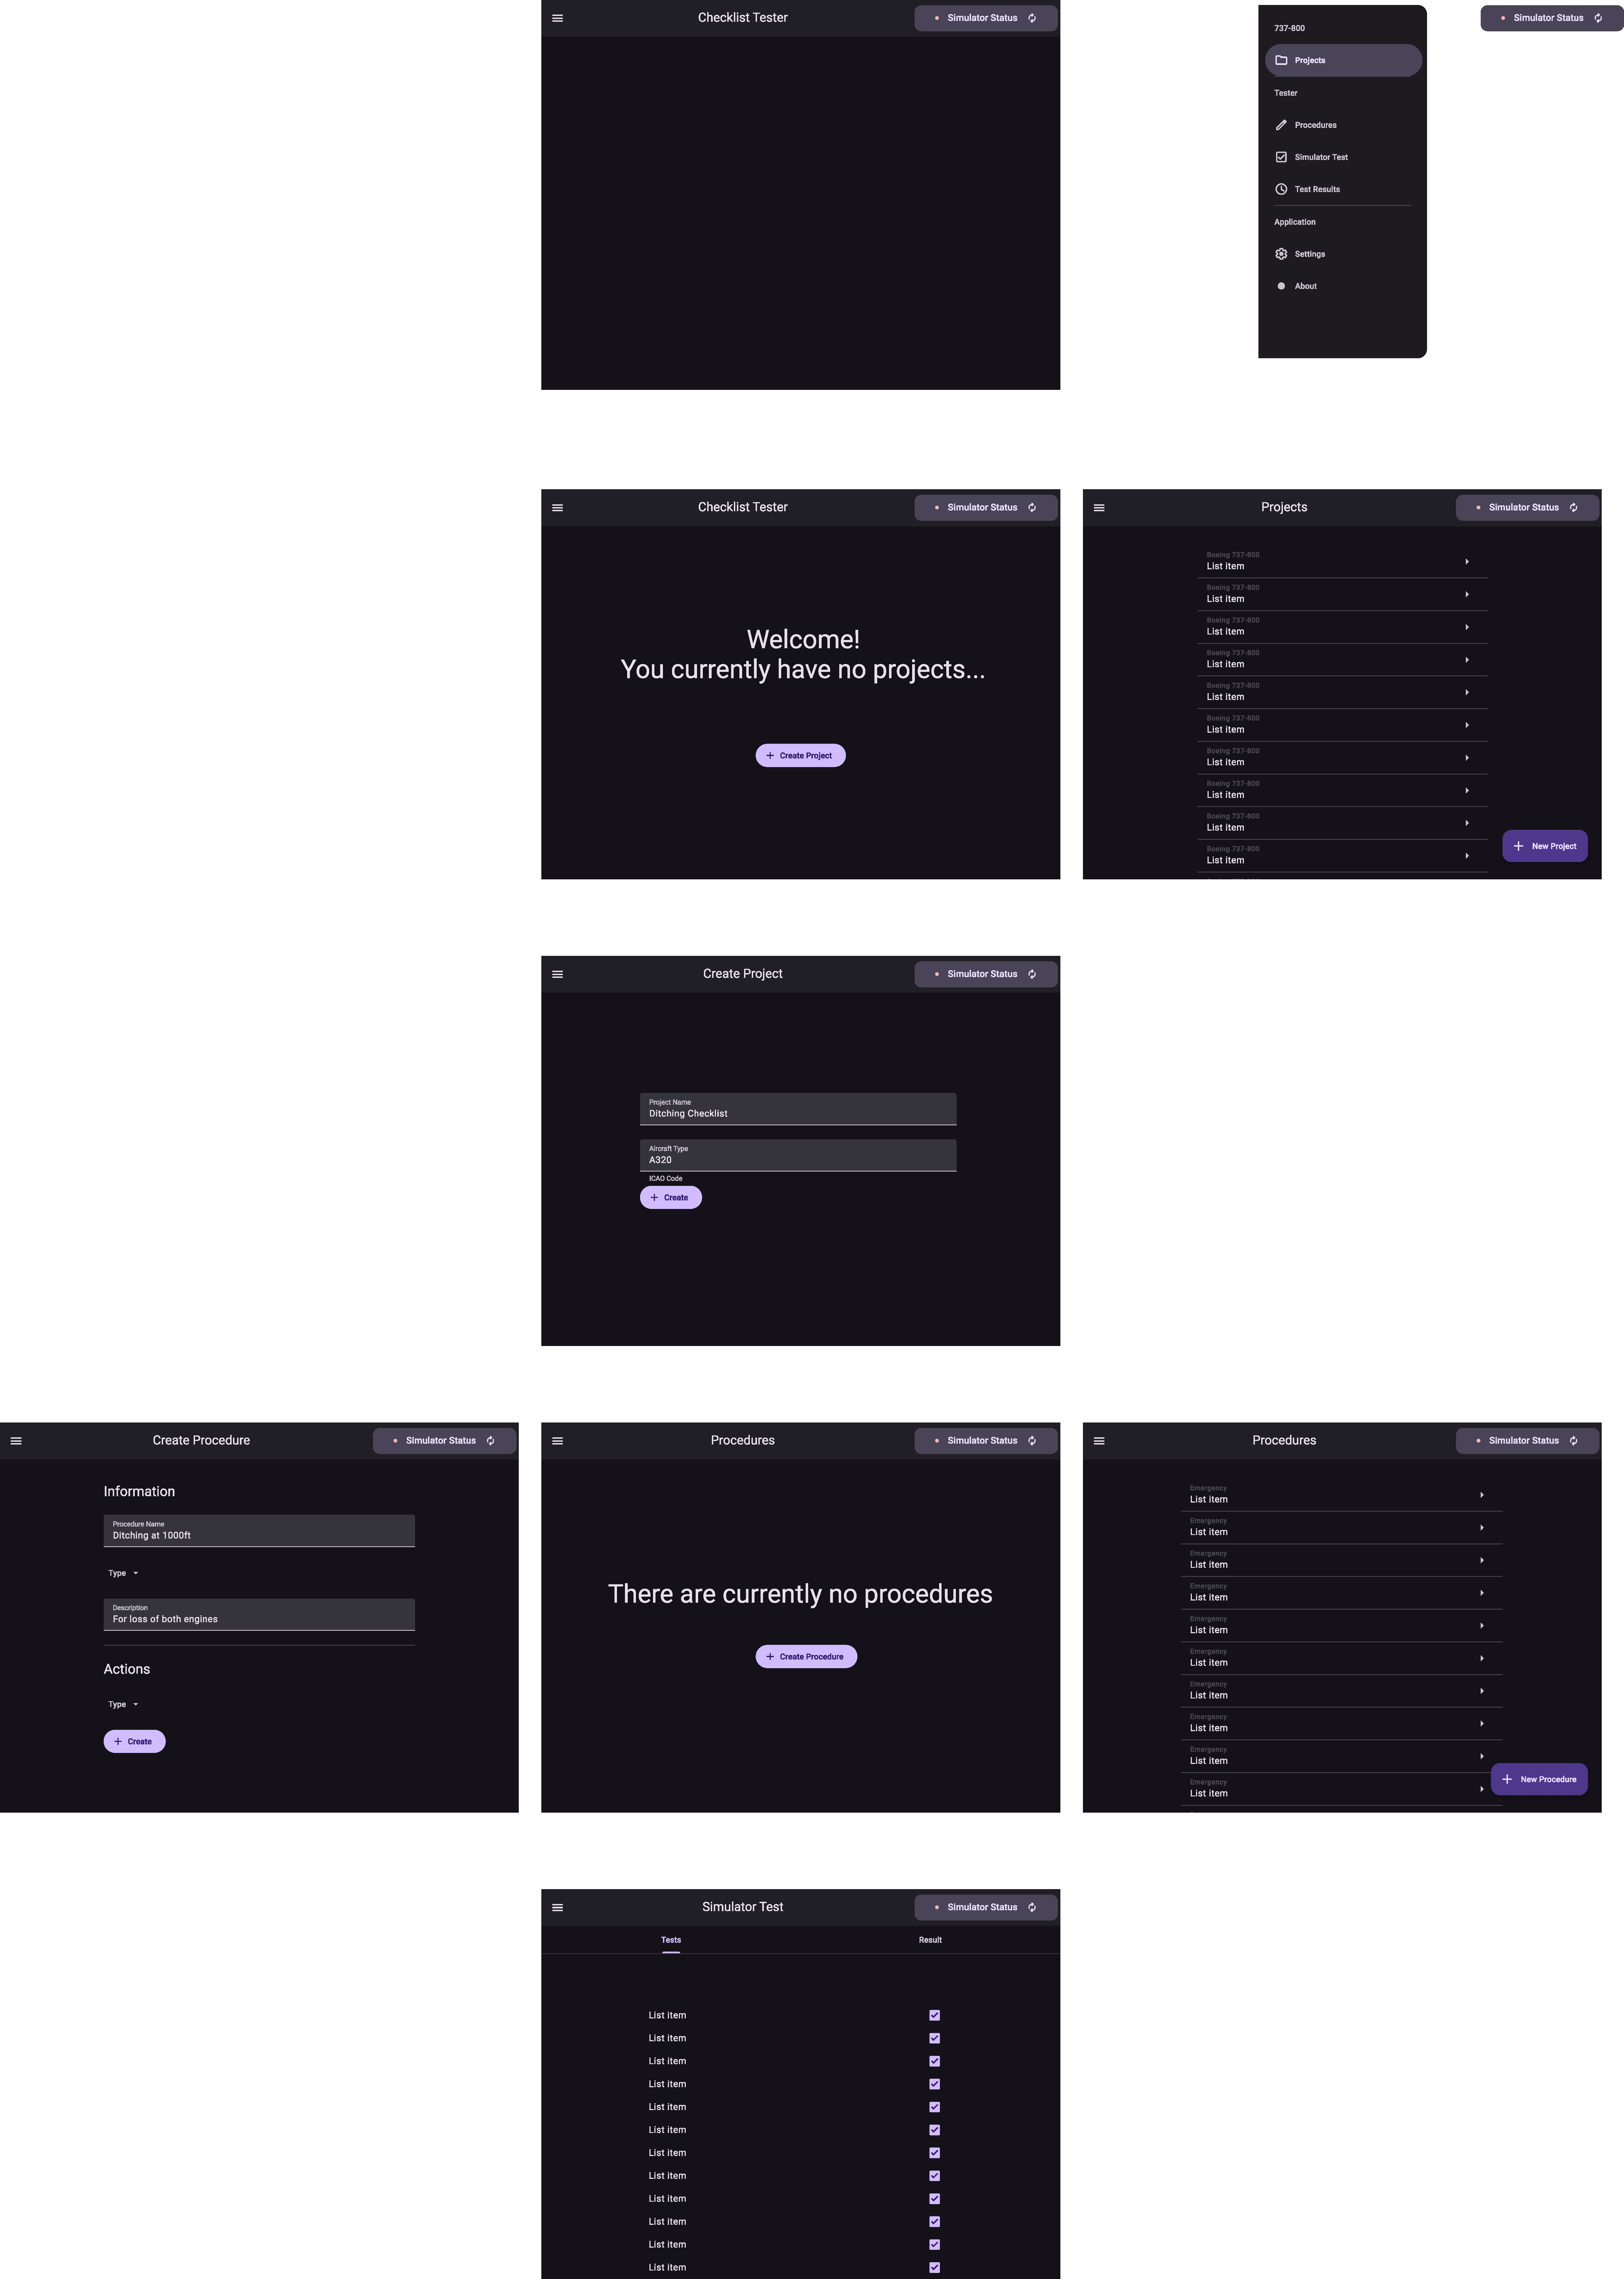
\includegraphics[width=\columnwidth]{images/figma-gui.pdf}
  \caption[GUI in Figma]{Design for the Checklist Connector GUI in Figma}
  \label{fig:figma-gui}
\end{figure}

\subsubsection{Limitations of Figma}
\begin{itemize}
  \item The Material 3 Components in Figma do not include features that are available in
    Jetpack Compose
  \item In this project, the \enquote{Simulator Test} at the bottom of Figure~\ref{fig:figma-gui}
    does not include a leading icon~\cite{material:lists}, and therefore had to be a trailing
    checkbox
  \item This was overcome by adding comments in Figma as a reminder of how the actual implementation
    should be like
  \item Another limitation is that in Figure~\ref{fig:figma-gui}, the title of the screen in the
    top app bar~\cite{material:top-app-bar} is not centered, and that is because the auto layout
    feature in Figma allows for equal spacing, rather than having each in a set position
\end{itemize}


\subsection{Compose Multiplatform}
\subsubsection{Setup}
\begin{itemize}
  \item Used the \textit{Kotlin Multiplatform Wizard} to create projects as it allows
    for runtime environments to be specified (in this case, Desktop and Server)
  \item Provides necessary build configurations in Gradle
  \item Planning what to implement important as Compose is designed to use modular
    components, otherwise a nested mess would occur as Compose is designed to have
    Composable functions passed in to a Composable function and therefore by design
    function nests will occur and the code will be harder to read if not managed correctly.
    Listing~\ref{list:compose-modular} shows example of using modular code
    from the Actions screen in project (with code omissions shown in comments)
  \item Used Voyager~\cite{voyager} to handle screens
  \item Used Koin~\cite{koin} for dependency injection, to be able to get data from the
    database and VDMJ
    \begin{itemize}
      \item Chose to use it because of Voyager integration with Koin~\cite{voyager:koin}
      \item Required as the application will be unresponsive when making requests
        to the database and/or VDMJ
      \item Used asynchronous coroutines to prevent the program from being blocked
    \end{itemize}
\end{itemize}

\begin{listing}
\inputminted[
  linenos,
  breaklines,
]{kotlin}{code/compose-modular.kt}
\caption{Example of modular code in Compose}
\label{list:compose-modular}
\end{listing}

\subsection{Storing Data}
\begin{itemize}
  \item Used SQLite databse with SQLDelight which creates typesafe Kotlin APIs
    to interact with the database
\end{itemize}
\begin{figure}[H]
  \centering
  \begin{tikzpicture}[
    auto,
    node distance = 1.5cm
  ]
    % PROCEDURE
    \node[entity] (procedure) {Procedure}
      [grow=up, sibling distance=2.25cm]
      child[grow=down] {node[attribute] {\textbf{id}}}
      child {node[attribute] {name}}
      child {node[attribute] {type}}
      child [grow=north west, level distance=2.15cm]{node[attribute] {description}}
      child [grow=right, level distance=3cm] {node[attribute] {createdUTC}}
      child [grow=left, level distance=3cm] {node[attribute] {modifiedUTC}};

    \node[relationship] (procProj) [above = of procedure] {Contains};

    % PROJECT
    \node[entity] (project) [right = of procProj] {Project}
      [grow=up, sibling distance=2cm]
      child {node[attribute] {name}}
      child {node[attribute] {\textbf{id}}}
      child {node[attribute] {aircraftType}}
      child[grow=right, level distance=3cm] {node[attribute] {createdUTC}}
      child[grow=south east, level distance=3cm] {node[attribute] {modifiedUTC}};

    \node[relationship] (procAct) [below left = of procedure] {Contains};

    % ACTION
    \node[entity] (action) [below left = of procAct] {Action}
      child[grow=up, level distance=2cm] {node[attribute] {step}}
      child[grow=right, level distance=2cm] {node[attribute] {\textbf{id}}}
      child[grow=north west, level distance=2cm] {node[attribute] {type}}
      child[grow=down, level distance=2cm] {node[attribute] {goal}};

    \node[relationship] (actionResult) [below right = of action] {Contains};

    % ACTION RESULT
    \node[entity] (result) [below right = of actionResult] {ActionResult}
      child[grow=up, level distance=2cm] {node[attribute] {\textbf{id}}}
      child[grow=left, level distance=3cm] {node[attribute] {startUTC}}
      child[grow=right, level distance=3cm] {node[attribute] {endUTC}}
      child[grow=south west, level distance=2cm] {node[attribute] {initState}}
      child[grow=south east, level distance=2cm] {node[attribute] {endState}};

    \node[relationship] (testAR) [above right = of result] {Contains};

    % TEST
    \node[relationship] (procTest) [below right = of procedure] {Contains};
 
    \node[entity] (test) [above right = of testAR] {Test}
      child[grow=left, level distance=2cm] {node[attribute] {\textbf{id}}}
      child[grow=north east, level distance=2cm] {node[attribute] {startUTC}}
      child[grow=south east, level distance=2cm] {node[attribute] {endUTC}};

    % RELATIONSHIP PATHS
    \path (procProj) edge node {\(N\)} (procedure)
      edge node {1} (project);

    \path (procTest) edge node {1} (procedure)
      edge node {\(N\)} (test);

    \path (procAct) edge node {1} (procedure)
      edge node {\(N\)} (action);

    \path (actionResult) edge node {1} (action)
      edge node {\(N\)} (result);

    \path (testAR) edge node {1} (test)
      edge node {\(N\)} (result);
  \end{tikzpicture}
  \caption[Connector ER Diagram]{Entity Relationship Diagram for the database in Checklist Connector}
  \label{fig:db-erd}
\end{figure}

\subsection{VDMJ Wrapper}


% Talk about how XPC was used here, not how it was implemented
\subsection{Connecting to the Flight Simulator}


\subsection{Testing}




%%%%% Simulator Connector Plugin %%%%%
\section{Simulator Connector Plugin}
% Talk about creating your own (originally happened) vs using something else that was developed
% Maybe talk about original plan? i.e. <project root>/plugin


\subsection{Creating Maven Package}
% Gradle
% Testing
% GitHub CI
\begin{itemize}
  \item XPC package is not published on a public Maven repository
  \item There has been a pull request that was merged to the \textit{develop} branch
    that provides Maven POMs~\cite{xpc:pom}. However, the maintainer for the
    project, at the time, did not have enough time to figure out the process of
    publishing the package to a Maven repository~\cite{xpc:pom-time}
  \item Therefore, had to find an alternative way to implement
  \item Jitpack~\cite{jitpack}
  \begin{itemize}
    \item In theory, simple to publish a repository, all that is required is a GitHub
      repository and searching if one has already been created on JitPack or build and publish
      a specific version
    \item However, due to the structure of the XPC repository, JitPack could not locate the
      build tools (Apache Maven in this case) as JitPack only searches on the root directory
      for the compatible build tools
  \end{itemize}
  \item Gradle gitRepository~\cite{gradle:gitRepository}
  \begin{itemize}
    \item There was not a lot of documentation
    \item Ambiguous on how to define directory for where the Java library is located in the Git repository
    \item However, as XPC was only built with Maven, Gradle was not able add the dependency as \lstinline|gitRepository()|
      only works with Gradle builds~\cite{gradle:gitRepoGradleOnly}
  \end{itemize}
\item Resorted to using a compiled Jar file and adding the dependency to Gradle
\item Not happy about that because it means maintaining it will be more difficult as
  it is not as simple as just changing the version number
\item Later, resorted to adding Gradle build files to XPC
\item Used automatic conversion from Maven to Gradle using \lstinline|gradle init| command~\cite{gradle:migratePOM}
\item Had to add local dependencies due to how Gradle works differently
\item Had to fix previous structure of Maven POM as the grouping as not good
\end{itemize}


\subsection{Submitting a Pull Request}
% What I did:
% - gitignore
% - changing url for repo
% - testing everything still worked




%%%%% SCENARIOS %%%%%
\section{Scenarios}
\begin{itemize}
  \item Use a Quick Reference Handbook (QRH) to find potential list of checklists to test
  % TODO find these accident reports
  \item Look at previous accident reports that had an incident related to checklists
    and test it with my tool to see if it will pick it up
  \item These previous accident reports can be good metrics to know what statistics to
    look out for
\end{itemize}


%%%%% DECISIONS %%%%%
\section{Decisions}
\end{document}
